\section{Thermodynamique d'une réaction électrochimique}
\subsection{Enthalpie libre de réaction}
Pour une réaction électrochimique, les potentiels des couples redox sont liés à l'enthalpie libre de réaction.

\formule{Enthalpie libre de réaction}
[]
{$$\Delta_rG=-n\mathcal{F}U$$}
[
    \begin{itemize}
        \item $\Delta_rG$ l'enthalpie libre de réaction (en \unit{J.mol^{-1}})
        \item $n$ le nombre d'électrons échangés (sans unité)
        \item $U=E_{+}-E_{-}$ la différence des potentiels des couples\footnote{$E_+$ correspond au potentiel du couple dont l'oxydant est coté réactif.} (en \unit{V})
        \item $\mathcal{F}=\mathcal{N}_ae$ la constante de Faraday (en \unit{C.mol^{-1}})
        \item $\mathcal{N}_a=\SI{6.02e23}{mol^{-a}}$ la constante d'Avogadro.
        \item $e=\SI{1.6e-19}{C}$ la charge élémentaire
    \end{itemize}
][o]

\flashcard{Enthalpie libre de réaction pour une réaction électrochimique}{$$\Delta_rG=-n\mathcal{F}U$$}

\application{Déterminer l'enthalpie libre de réaction de \ce{2 Fe^2+ + 2 Zn -> 2 Fe^2+ + Zn^2+}. On donne $\ce{[Fe^2+]}=\ce{[Fe^3+]}=\ce{[Zn^2+]}=\SI{0.1}{mol.L^{-1}}$ et $E^\circ(\ce{Fe^3+/Fe^2+})=\SI{0.77}{V}$ et $E^\circ(\ce{Zn^2+/Zn})=\SI{-0.7628}{V}$}

\application{Déterminer l'enthalpie libre standard de réaction de la réaction précédente.}

\application{Écrire la réaction d'oxydoréduction faisant intervenir les couples \ce{O2/H2O} et \ce{H2O/H2}. En déduire le potentiel standard du couple \ce{O2 / H2O} à la température de référence.
\begin{tabular}{c|c|c|c}
    & \ce{H2O (l)} & \ce{H2} & \ce{O2} \\
    $\Delta_fH^\circ$ (\unit{kJ/mol}) & \num{-241.8} & & \\
    $S_m$ (\unit{J/mol/K}) & \num{188.74} & \num{130.46} & \num{204.82} \\
\end{tabular}
}

\subsection{Travail électrique}

Le travail électrique reçu par un un système chimique est borné par la variation d'enthalpie libre.

\formule{Travail électrique}
[
    \begin{itemize}
        \item Pour une transformation isotherme isobare.
        \item Les seuls travaux sont les travaux électriques et les travaux des forces de pression.
    \end{itemize}
]
{$$-W\leq\Delta G$$}
[
    \begin{itemize}
        \item $W$ le travail reçu par le système chimique (en \unit{J})
        \item $\Delta G$ la variation d'enthalpie libre (en \unit{J})
    \end{itemize}
][o][o]

\formule{Travail maximal récupérable d'un système électrochimique}{$$-W\leq\Delta G$$}



\section{Réaction et courant électrique}
\subsection{Courant électrique}
Dans une pile ou un électrolyseur, la vitesse de réaction est liée au courant électrique.

\formule{Courant électrique}
[La réaction électrochimique s'effectue à la surface d'une électrode grace au courant arrivant à celle-ci.]
{$$i=-n\mathcal{F}\frac{d\xi}{dt}$$}
[
    \begin{itemize}
        \item $i$ le courant électrique \textbf{arrivant} à l'électrode (en \unit{A})
        \item $\mathcal{F}$ la constante de Faraday (en \unit{C.mol^{-1}})
        \item $\xi$ l'avancement (en \unit{mol})
    \end{itemize}
][o][o]

\formule{Courant rentrant à une électrode}{$$i=-n\mathcal{F}\frac{d\xi}{dt}$$}

On peut également définir $j=\frac{i}{S}$ la densité volumique de courant arrivant à l'électrode. avec $S$ la surface immergée de l'électrode.

\subsection{Montage à 3 électrodes}
Pour mesurer la valeur du courant $i$ rentrant dans l'électrode en fonction de son potentiel, on a recourt au montage à 3 électrodes.
\schema{Montage à trois électrodes}{5cm}

Le voltmètre mesure la différence de potentiels entre l'électrode de travail et l'électrode de référence. Cette dernière ayant un potentiel fixe et connu, on peut en déduire le potentiel $E$ de l'électrode de travail.

Comme il n'est pas possible de faire passer du courant dans une électrode de référence (risque de dommages et perte du caractère << de référence >>), on utiliser une troisième électrode appelée contre-électrode dont le rôle est de fermer le circuit.

Avec ce montage, on peut mesurer point par point la courbe $i(E)$.

\colle{Établir la relation entre courant arrivant à une électrode et vitesse de réaction. Schématiser le montage permettant de mesurer ce courant en fonction du potentiel en expliquant le role de chaque électrode.}

\subsection{Courbes intensité-potentiel}
Une courbe intensité potentiel représente l'intensité du courant arrivant à une électrode en fonction du potentiel électrique de l'électrode.

Une courbe intensité-potentiel dépend du couple redox, des concentrations et de l'électrode sur lequel il est tracé.

\schema{Allure d'une courbe intensité-potentiel}{4cm}

\exemple{Courbe intensité potentiel pour les courbes de l'eau sur une électrode de platine.
\begin{center}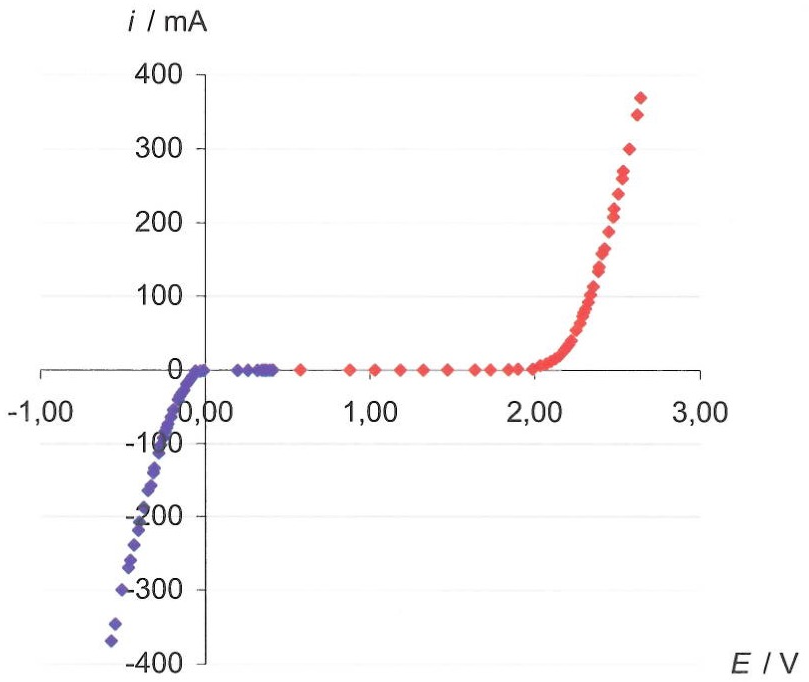
\includegraphics[height=4cm]{images/i-e.png}\end{center}}

Pour $i=0$, la réaction est à l'équilibre chimique : elle n'évolue ni dans un sens ni dans l'autre. Son potentiel $E_{eq}$ est donné par la formule de Nernst.

Pour $i>0$, la vitesse $v=-\frac{i}{n\mathcal{F}}<0$. La réaction évolue dans le sens indirect. L'électrode est une anode.

Pour $i<0$, la vitesse $v=-\frac{i}{n\mathcal{F}}>0$. La réaction évolue dans le sens direct. L'électrode est une cathode.

Expérimentalement, il n'est pas possible de savoir à quelle réaction chimiques participent les électrons qui sont mesurés par l'ampèremètre. Les courbes intensité-potentiel mesurées représentent la somme des courants pour toutes les réactions en cours.

\subsubsection{Système rapide et système lent}
Pour certaines réactions et sur certaines électrodes, un courant mesurable n'apparait pas forcément dès que le potentiel s'éloigne du potentiel d'équilibre. Il faut alors attendre d'avoir dépassé un certain écart appelé surpotentiel. On dit alors que le système est un système lent.

\schema{Système rapide et système lent}{4cm}

Remarque : La valeur du surpotentiel\footnote{Le surpotentiel est parfois appelé surtension.} dépend de la valeur arbitrairement choisie d'un << courant mesurable >>.

\subsubsection{Paliers de diffusion}
Les solutés sont transportés dans la solution par
\begin{itemize}
\item diffusion (dans la couche limite)
\item convection (en dehors de la couche limite)
\item migration (pour les ions)
\end{itemize}
En pratique, le phénomène de migration est négligeable.

Lorsque les courants gagnent entre intensité, les solutés nécessaires à la réaction peuvent venir à manquer au voisinage immédiat de l'électrode. Ils n'ont pas le temps de diffuser jusqu'à l'électrode, ce qui limite le courant. Des \textbf{paliers de diffusion} apparaissent alors sur la courbe.

\schema{Palier de diffusion}{4cm}

\formule{Courant sur un palier de diffusion}
[]
{$$i_\text{max}=\frac{n\mathcal{F}SDc}{\delta}$$}
[
    \begin{itemize}
        \item $i_\text{max}$ l'intensité du courant sur le palier de diffusion (en \unit{A})
        \item $n$ le nombre d'électrons échangés (sans dimension)
        \item $\mathcal{F}$ la constante de Faraday (en \unit{C.mol^{-1}})
        \item $S$ la surface immergée de l'électrode (en \unit{m^2})
        \item $D$ le coefficient de diffusion (en \unit{m^2.s^{-1}})
        \item $c$ la concentration de l'espèce limitant le courant (en \unit{mol.L^{-1}})
        \item $\delta$ l'épaisseur de la couche limite (en \unit{m})
    \end{itemize}
][][o]

\colle{Expriquer ce qu'est un palier de diffusion et dans quel cas il peut être présent. Exprimer la hauteur d'un palier de diffusion en fonction de la concentration et de l'épaisseur de la couche limite.}

Lorsque le réactif ne peut pas manquer à l'électrode (si c'est le solvant ou l'électrode elle-même), il n'y a pas de palier de diffusion.

\application{Parmi toutes les réactions ci-après, déterminer celles qui peuvent posséder un palier de diffusion sur leur courbe intensité-potentiel.\\\ce{Fe^{3+} + e^- -> Fe^{2+}}, \ce{Zn -> Zn^2+ + 2e-}, \ce{2H2O -> O2 + 2H+ + 2e-}, \ce{2H+ + 2e- -> H2}}

\subsubsection{Mur du solvant}
Si le solvant participe à au moins un couple redox, on peut tracer sa courbe intensité-potentiel, appelée mur du solvant.

C'est le cas de l'eau, qui intervient comme oxydant dans le couple \ce{H2O}/\ce{H2} ($E^\circ=\SI{0}{V}$) et comme réducteur dans le couple \ce{H2O}/\ce{O2} ($E^\circ=\SI{1.23}{V}$). Leur courbe dépend beaucoup de la nature de l'électrode qui catalyse plus ou moins la réaction, celle-ci est donc précisée sur la courbe.

\schema{Mur du solvant}{4cm}

\application{Tracer l'allure de la courbe intensité-potentiel d'une électrode d'argent dans une solution de nitrate d'argent à \SI{0.01}{mol.L^{-1}} acidifiée à $pH=1$. On fera figurer le mur du solvant, les éventuels paliers de diffusion et les éventuelles surpotentiels.\\$E^\circ(\ce{Ag+/Ag})=\SI{0.77}{V}$, surpotentiel de \ce{H2O/H2} sur l'argent : \SI{-0.22}{V}, surpotentiel de \ce{O2/H2O} sur l'argent : \SI{0.91}{V}, \ce{Ag+/Ag} est un couple rapide.}



\section{Piles, accumulateurs et électrolyseurs}
\subsection{Présentation et rappels}
Une pile est un dispositif permettant de convertir de l'énergie chimique en énergie électrique. Une pile utilise une réaction spontanée pour faire transiter des électrons dans un circuit électrique.

Lorsque cette conversion est réversible, on parle d'accumulateur\footnote{Dans la vie courante, on parle de batterie.}.

Une pile est constitué de deux demi piles. Un demi-pile est constitué d'une électrode plongée dans une solution.

\schema{Pile}{4cm}

\exemple{Pile alcaline, pile au lithium, pile Daniel.}

\exemple{Accumulateur Li-ion, accumulateur au plomb.}

Un électrolyseur est un dispositif permettant de convertir de l'énergie électrique en énergie chimique. Un électrolyseur utilise une tension pour forcer une réaction à se produire dans le sens opposé au sens spontané.

\exemple{Production de dihydrogène, d'aluminium.}

\subsection{Caractéristique}

Il est possible de construire la caractéristique d'une pile ou d'un électrolyseur à partir de la courbe intensité-potentiel de ses deux électrodes.

\application{On considère une pile Daniel constitué d'une électrode en cuivre et d'une électrode en zinc. Les courbes intensité-potentiel sont fournies ci-dessous. Quel courant maximale peut débiter la pile. Que vaut sa tension à vide ? Tracer la caractéristique courant-tension de la pile Daniel. On prendra les courants $\{0, 0.2, \SI{0.4}{A}\}$ pour le tracé et on fera également apparaitre la saturation en courant.\\
\begin{center}
    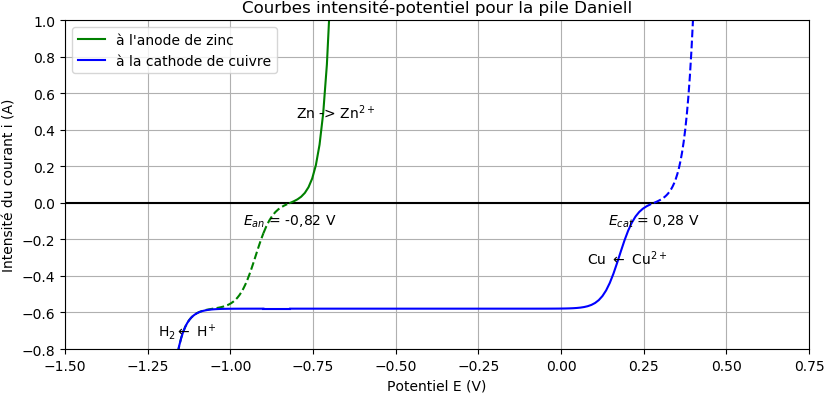
\includegraphics[width=.9\linewidth]{images/courbes_i-E_Daniell.png}
\end{center}
}

\application{Le procédé chlore-soude permet de produire de la soude, du dihydrogène et du dichlore à partir d'une solution de chlorure de sodium. Quelle tension minimale faut-il appliquer pour que la réaction voulue démarre ? Quel courant maximal peut-on faire passer dans cet électrolyseur ? Quelle tension imposer pour avoir un courant de \SI{200}{A} ?\\
\begin{center}
    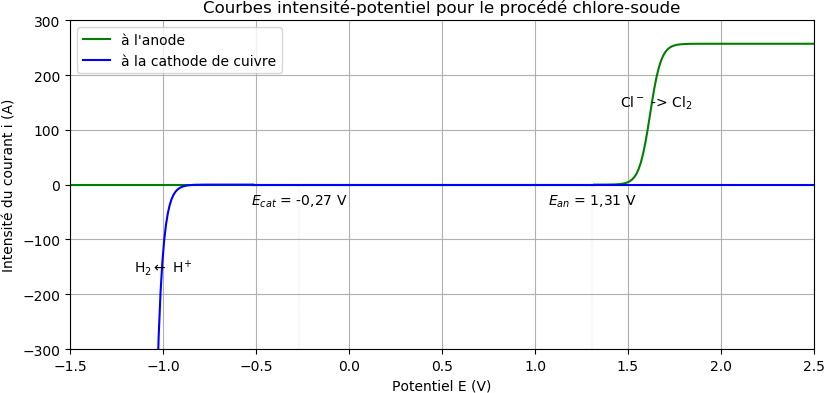
\includegraphics[width=.9\linewidth]{images/courbes_i-E_chlore-soude.png}
\end{center}
}

La tension effectivement mesurée aux bornes d'une pile peut être plus faible que la tension prévue par les courbes intensité-potentiel. Ce phénomène s'explique par la présence d'une résistance interne dans la pile qui est essentiellement due au pont ionique séparant les deux demi-piles. La résistance interne est d'autant plus faible que les ions sont mobiles, que le pont salin est cours et que les ions sont concentrés.

\subsection{Capacité et masse électrolysée}
La capacité d'une pile\footnote{Attention, la capacité d'une pile n'a rien à voir avec la capacité d'un condensateur, bien que le terme utilisé soit le même. Ces grandeurs n'ont même pas la même unité.} est la quantité d'électricité qu'elle peut débiter avant d'atteindre l'équilibre chimique. La capacité d'une pile se mesure en \unit{C}. Les capacités sont usuellement données en \unit{A.h} (\SI{1}{A.h}=\SI{3600}{C}).

La capacité d'une pile peut être déduite d'un tableau d'avancement.

\application{On s'intéresse à une pile Daniell constituée des deux demi-piles suivantes.
\begin{itemize}
    \item Une électrode de cuivre dans \SI{100}{mL} d'une solution de sulfate de cuivre à \SI{1}{mol.L^{-1}}
    \item Une électrode de zinc dans \SI{100}{mL} d'une solution de sulfate de zinc à \SI{1}{mol.L^{-1}}
\end{itemize}
Déterminer l'avancement lorsque l'équilibre chimique est atteint. En déduire la capacité de la pile.\\
Données : $E^\circ(\ce{Cu^2+/Cu}) = \SI{0.340}{V}$ ; $E^\circ(\ce{Zn^2+/Zn}) = \SI{-0.7618}{V}$.
}

Le même raisonnement peut être utilisé pour déterminer la masse électrolysée.

\application{Un électrolyseur industriel permet de produire \SI{7}{kg} de \ce{Al (s)} par jour à partir de \ce{Al^3+ (aq)}. Déterminer le courant passant dans l'électrolyseur en supposant qu'il n'y a pas de réactions parasites.\\
Donnée : $M(\ce{Al})=\SI{27}{g.mol^{-1}}$}

\subsection{Rendement faradique}
Le \textbf{rendement faradique} est la proportion des électrons participant à le réaction chimique désirée.

\flashcard{Rendement faradique}{Proportion du courant participant à la réaction désirée.}

\application{En réalité, le courant est de \SI{1000}{A} dans l'électrolyseur précédant. Déterminer le rendement faradique.}




\section{Corrosion humide}
\subsection{Présentation}
La corrosion est un phénomène par lequel les métaux et les alliages subissent une attaque de leur environnement qui les fait évoluer à l'état d'ions métalliques par une réaction d'oxydation. Le dioxygène dissous et l'eau sont les deux principaux agents oxydants.

La corrosion est d'autant plus rapide que le solvant est riche en ions et en dioxygène. La présence de microorganismes favorise également la corrosion. Les infrastructure navales et les bateaux sont particulièrement sujet à la corrosion.

\subsection{Corrosion uniforme}
On parle de corrosion uniforme lorsque l'intégralité de la pièce métallique est corrodée de façon homogène sur sa surface. Elle se produit en solution acide ou en solution neutre oxygénée.
\exemple{En milieu acide : \ce{Fe(s) + 2H+(aq) -> Fe^{2+}(aq) + H2(g)} le fer est corrodé.}

\subsubsection{Aspect thermodynamique}
L'existence de phénomène de corrosion peut être déduite de la superposition du diagramme potentiel-pH du métal avec celui de l'eau. Trois cas sont possibles :
\begin{description}
    \item[Domaine d'immunité] Le métal a un domaine commun avec l'eau. Aucune réaction ne se produit. Le métal n'est pas corrodé.
    \item[Dommaine de corrosion] Le métal n'a pas de domaine commun avec l'eau et l'espèce formée est un ion. Le métal est corrodé. La réaction électrochimique se poursuit jusqu'à disparition du métal.
    \item[Domaine de passivation]  Le métal n'a pas de domaine commun avec l'eau et l'espèce formée est un solide. La surface du métal réagit mais le solide formé protège\footnote{Cette protection n'est pas totale. Par exemple, pour le fer, l'oxyde de fer III (la rouille) est poreuse et laisse passer l'eau qui oxyde le fer en profondeur.} le reste du métal de tout contact avec le solvant. La réaction s'arrête dès que la passivation a eu lieu.
\end{description}

\begin{figure}[!ht]
    \begin{subfigure}{.45\linewidth}
        \centering
        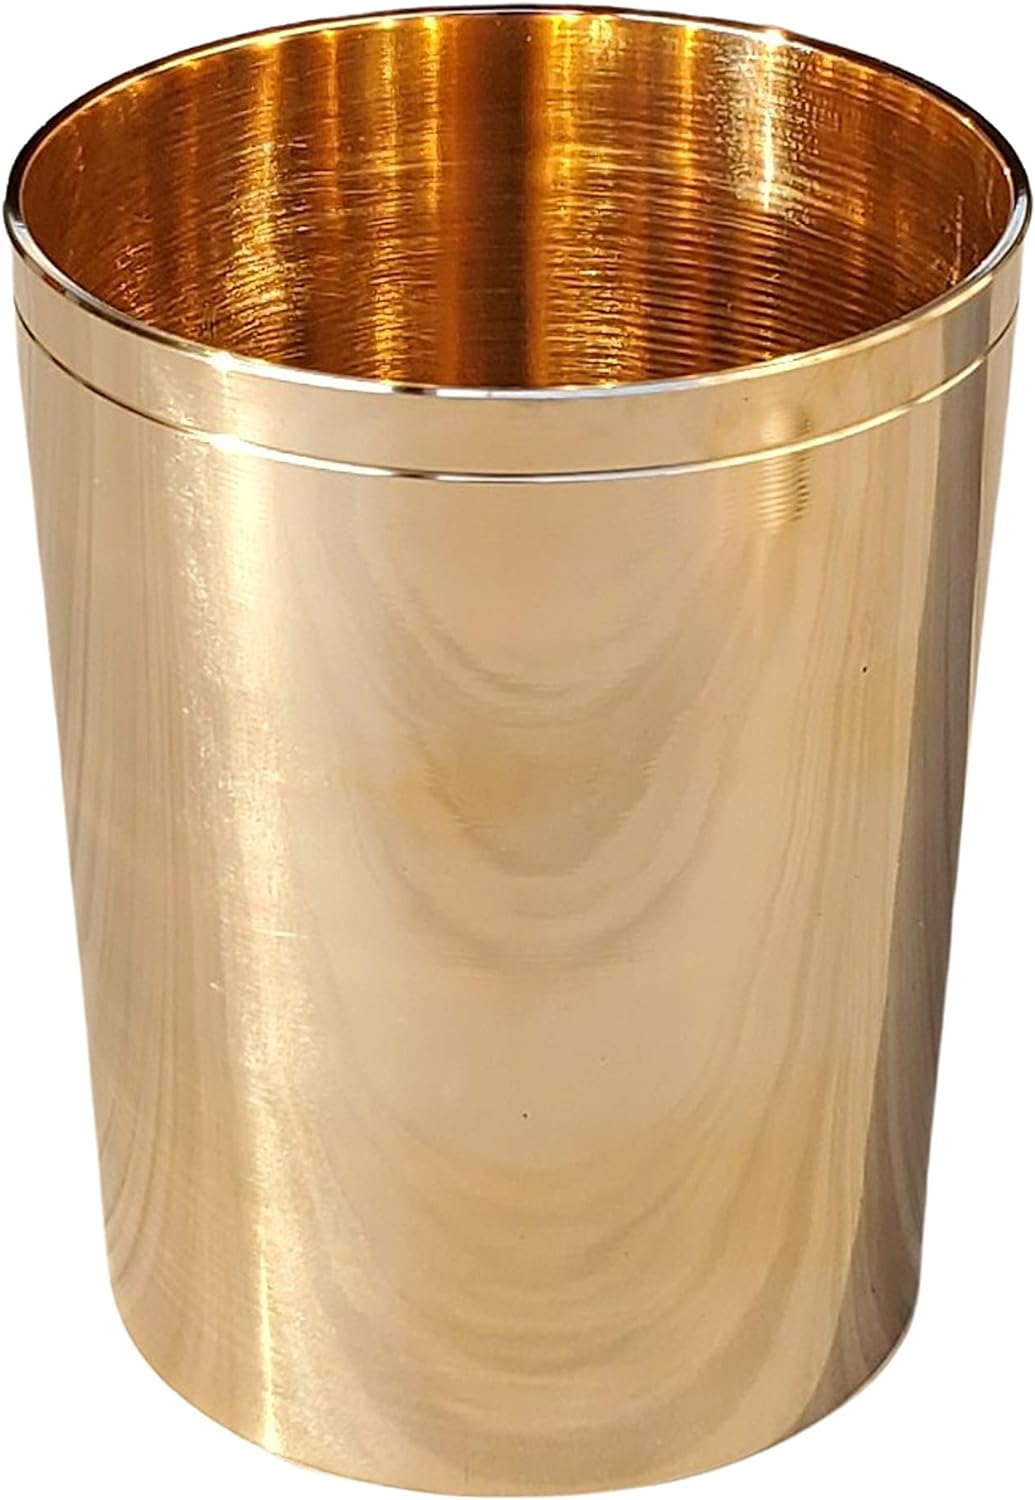
\includegraphics[height=5cm]{images/bronze1.jpg}
        \caption{Bronze poli.}
    \end{subfigure}
    \hfill
    \begin{subfigure}{.45\linewidth}
        \centering
        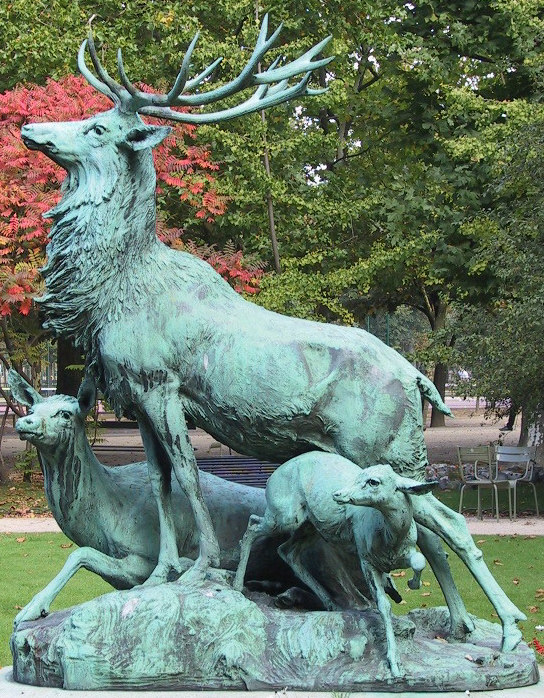
\includegraphics[height=5cm]{images/bronze2.jpg}
        \caption{Bronze recouvert d'une couche de vert de gris par passivation naturelle.}
    \end{subfigure}
\end{figure}

\application{Déterminer pour le fer, l'or et l'alumimum et en fonction du pH, si on a immunité, passivation ou corrosion. Les traits en pointillés représentent les courbes potentiel-pH de l'eau.\\
\begin{center}
    \includesvg[height=7cm]{images/EpH-Fe.svg}\\
    \includesvg[height=7cm]{images/EpH-Au.svg}\hfill
    \includesvg[height=7cm]{images/EpH-Al.svg}
\end{center}}

\subsubsection{Aspect cinétique}
La cinétique des phénomènes de corrosion peut être déduite des courbes intensité-potentiel.

L'oxydation et la réduction s'effectuant au même endroit, il n'y a qu'un seul potentiel, appelé potentiel de corrosion. Le potentiel de corrosion est un cas particulier de potentiel mixte. L'électrode reste électriquement neutre donc il y a autant d'électrons produits par l'oxydation que consommés par la réduction, les courants anodiques et cathodiques sont donc égaux. Un seul point des courbes intensité-potentiel vérifient ces conditions.

\schema{Potentiel de corrosion}{5cm}


\subsection{Corrosion différentielle}
La corrosion différentielle apparait lorsque deux pièces métalliques différentes sont en contact ou que le milieu est inhomogène. On parle de pile de corrosion.

L'oxydation et la réduction se font donc à des endroits différents.

\exemple{Corrosion du zinc en présence de fer.\\\\
\includesvg[height=7cm]{images/i-E Fe Zn.svg}}


\subsection{Protection contre la corrosion}

Il existe différentes techniques pour protéger un métal de la corrosion.

\subsubsection{Recouvrement}
On peut recouvrir le métal d'une substance étanche pour empêcher le contact avec l'eau.

La substance peut être de la peinture, un métal (chromage, galvanisation, ...) ou un oxyde métallique.

La passivation peut être naturelle lorsque la réaction se fait spontanément en contact de l'eau ou forcée si elle est faite par électrolyse.

\exemple{La passivation du zinc et de l'aluminium sont naturelle.}

\subsubsection{Anode sacrificielle}

La protection par anode sacrificielle consiste à réaliser volontairement une pile de corrosion en mettant la pièce à protéger en contact avec une anode. La pièce à protéger sera alors une cathode et une oxydation ne pourra pas s'y produite.

\schema{Protecion par anode sacrificeille}{4cm}

\begin{figure}[!ht]
    \begin{subfigure}[t]{.3\linewidth}
        \centering
        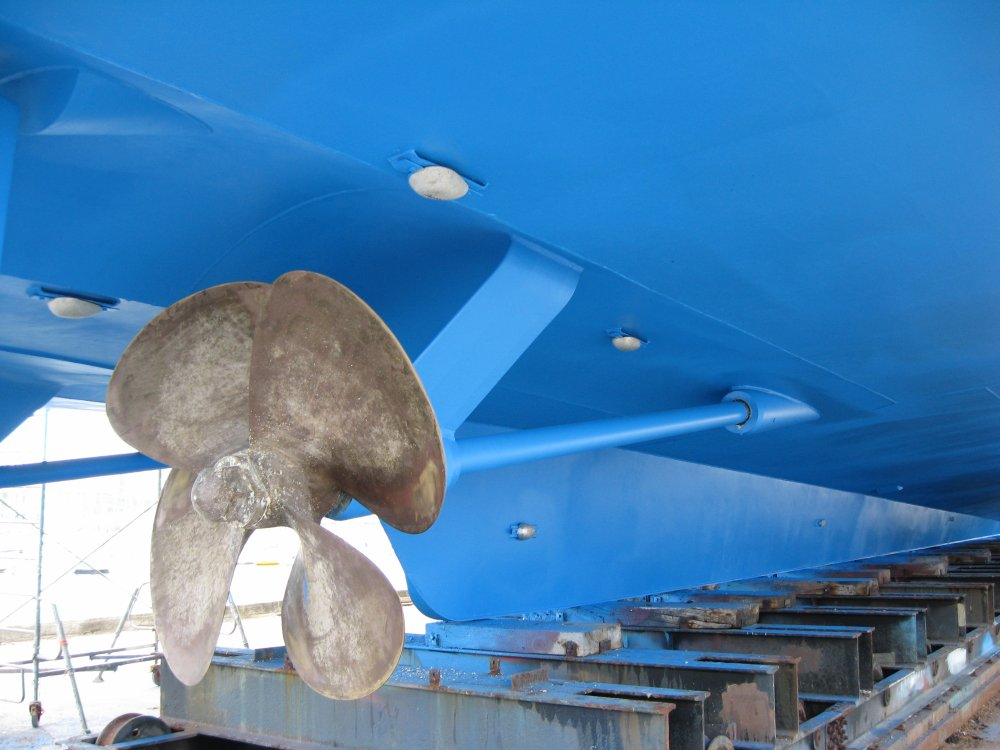
\includegraphics[height=4cm]{images/bateau1.jpg}
        \caption{Anodes sacrificielles en places.}
    \end{subfigure}
    \hfill
    \begin{subfigure}[t]{.3\linewidth}
        \centering
        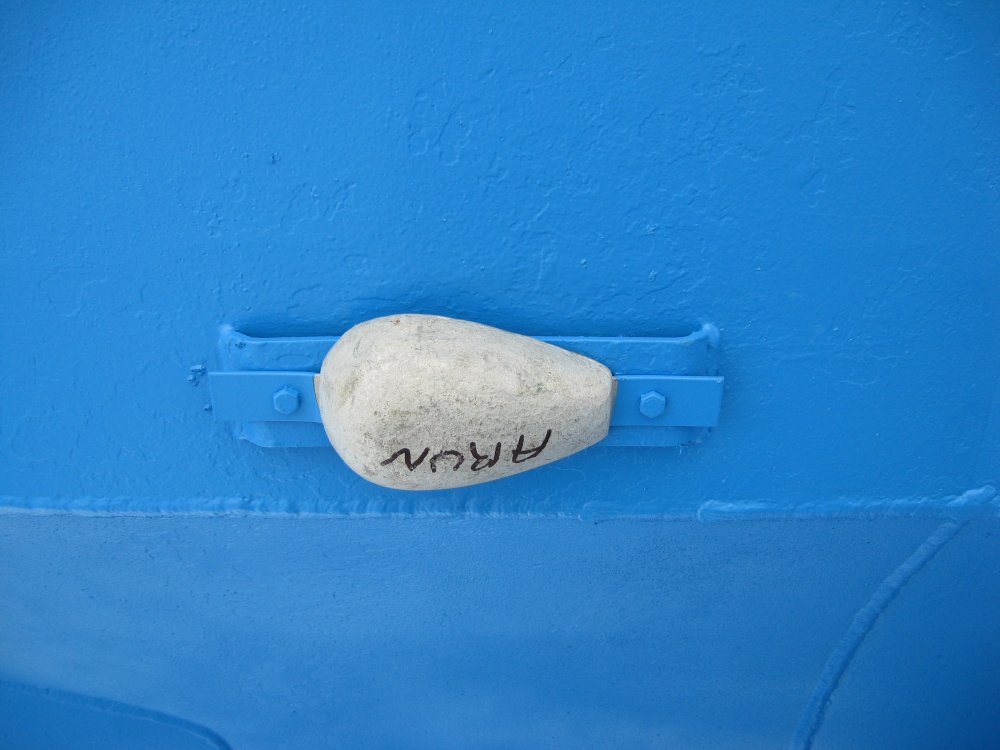
\includegraphics[height=4cm]{images/bateau2.jpg}
        \caption{Détail des anode sacrificielles neuves.}
    \end{subfigure}
    \hfill
    \begin{subfigure}[t]{.3\linewidth}
        \centering
        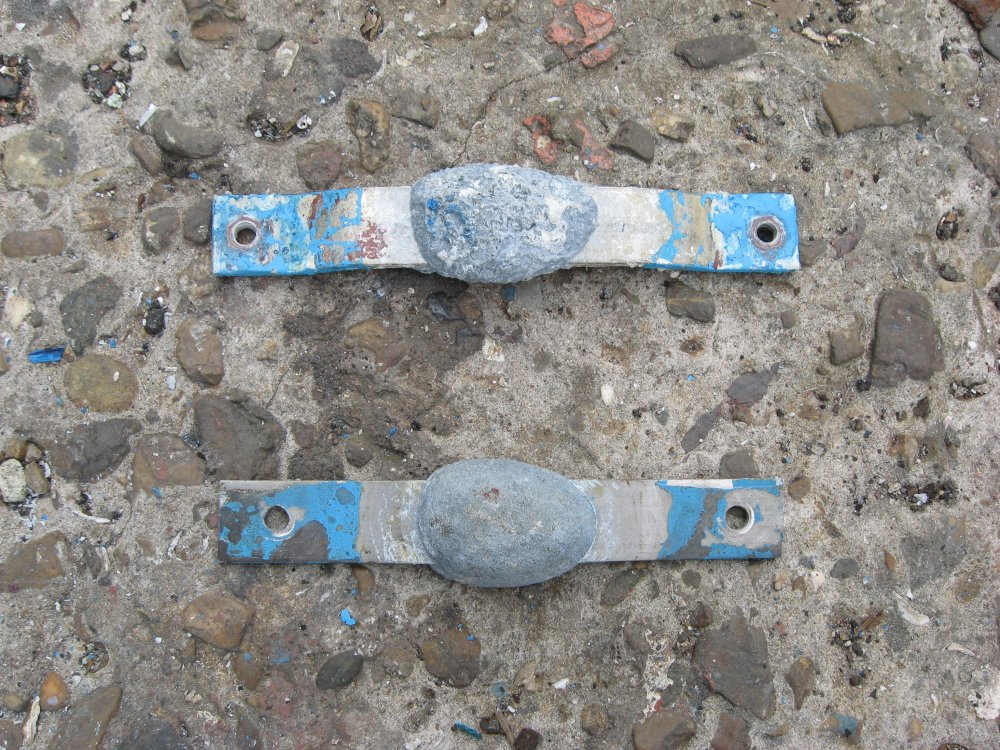
\includegraphics[height=4cm]{images/bateau3.jpg}
        \caption{Anodes sacrificielles usées.}
    \end{subfigure}
    \caption{Anodes sacrificielles en zinc installées sur un bateau.}
\end{figure}

\exemple{La galvanisation (recouvrir une pièce en acier par une fine couche de zinc) permet de protéger l'acier par recouvrement, et, en cas de raillure, l'acier et toujours protégé car le zinc joue le role d'anode sacrificielle.}

\subsubsection{Courant imposé}
La protection par courant imposé consiste à imposer un courant pour contrôler les réactions se produisant à l'électrode à protéger. 

La protection cathodique consiste à augmenter le potentiel pour empêcher l'oxydation de se produire.

La protection anodique consiste à diminuer le potentiel pour forcer une réaction de passivation à se produire.

\colle{Présenter 3 méthodes permettant de protéger un métal de la corrosion.}